\section{Resultados}
La configuración inicial que se le dio a cada sistema esta dado por las siguientes ecuaciones:
\begin{align*}
    x_{i+1}&=(i-1)*0.9+a\\
    y_{i+1}&=\left\lbrace\begin{matrix}
        0.5+a & mod(i,2)=0 \\
        a & mod(i,2)\neq 0
    \end{matrix} \right.
\end{align*}
donde a representa un número aleatorio entre -0.1 y 0.1. Con ello, las configuraciones iniciales de cada ejecución del modelo estan
mostradas en la figura \ref{fig:posini}.
\begin{figure}[H]
    \centering
    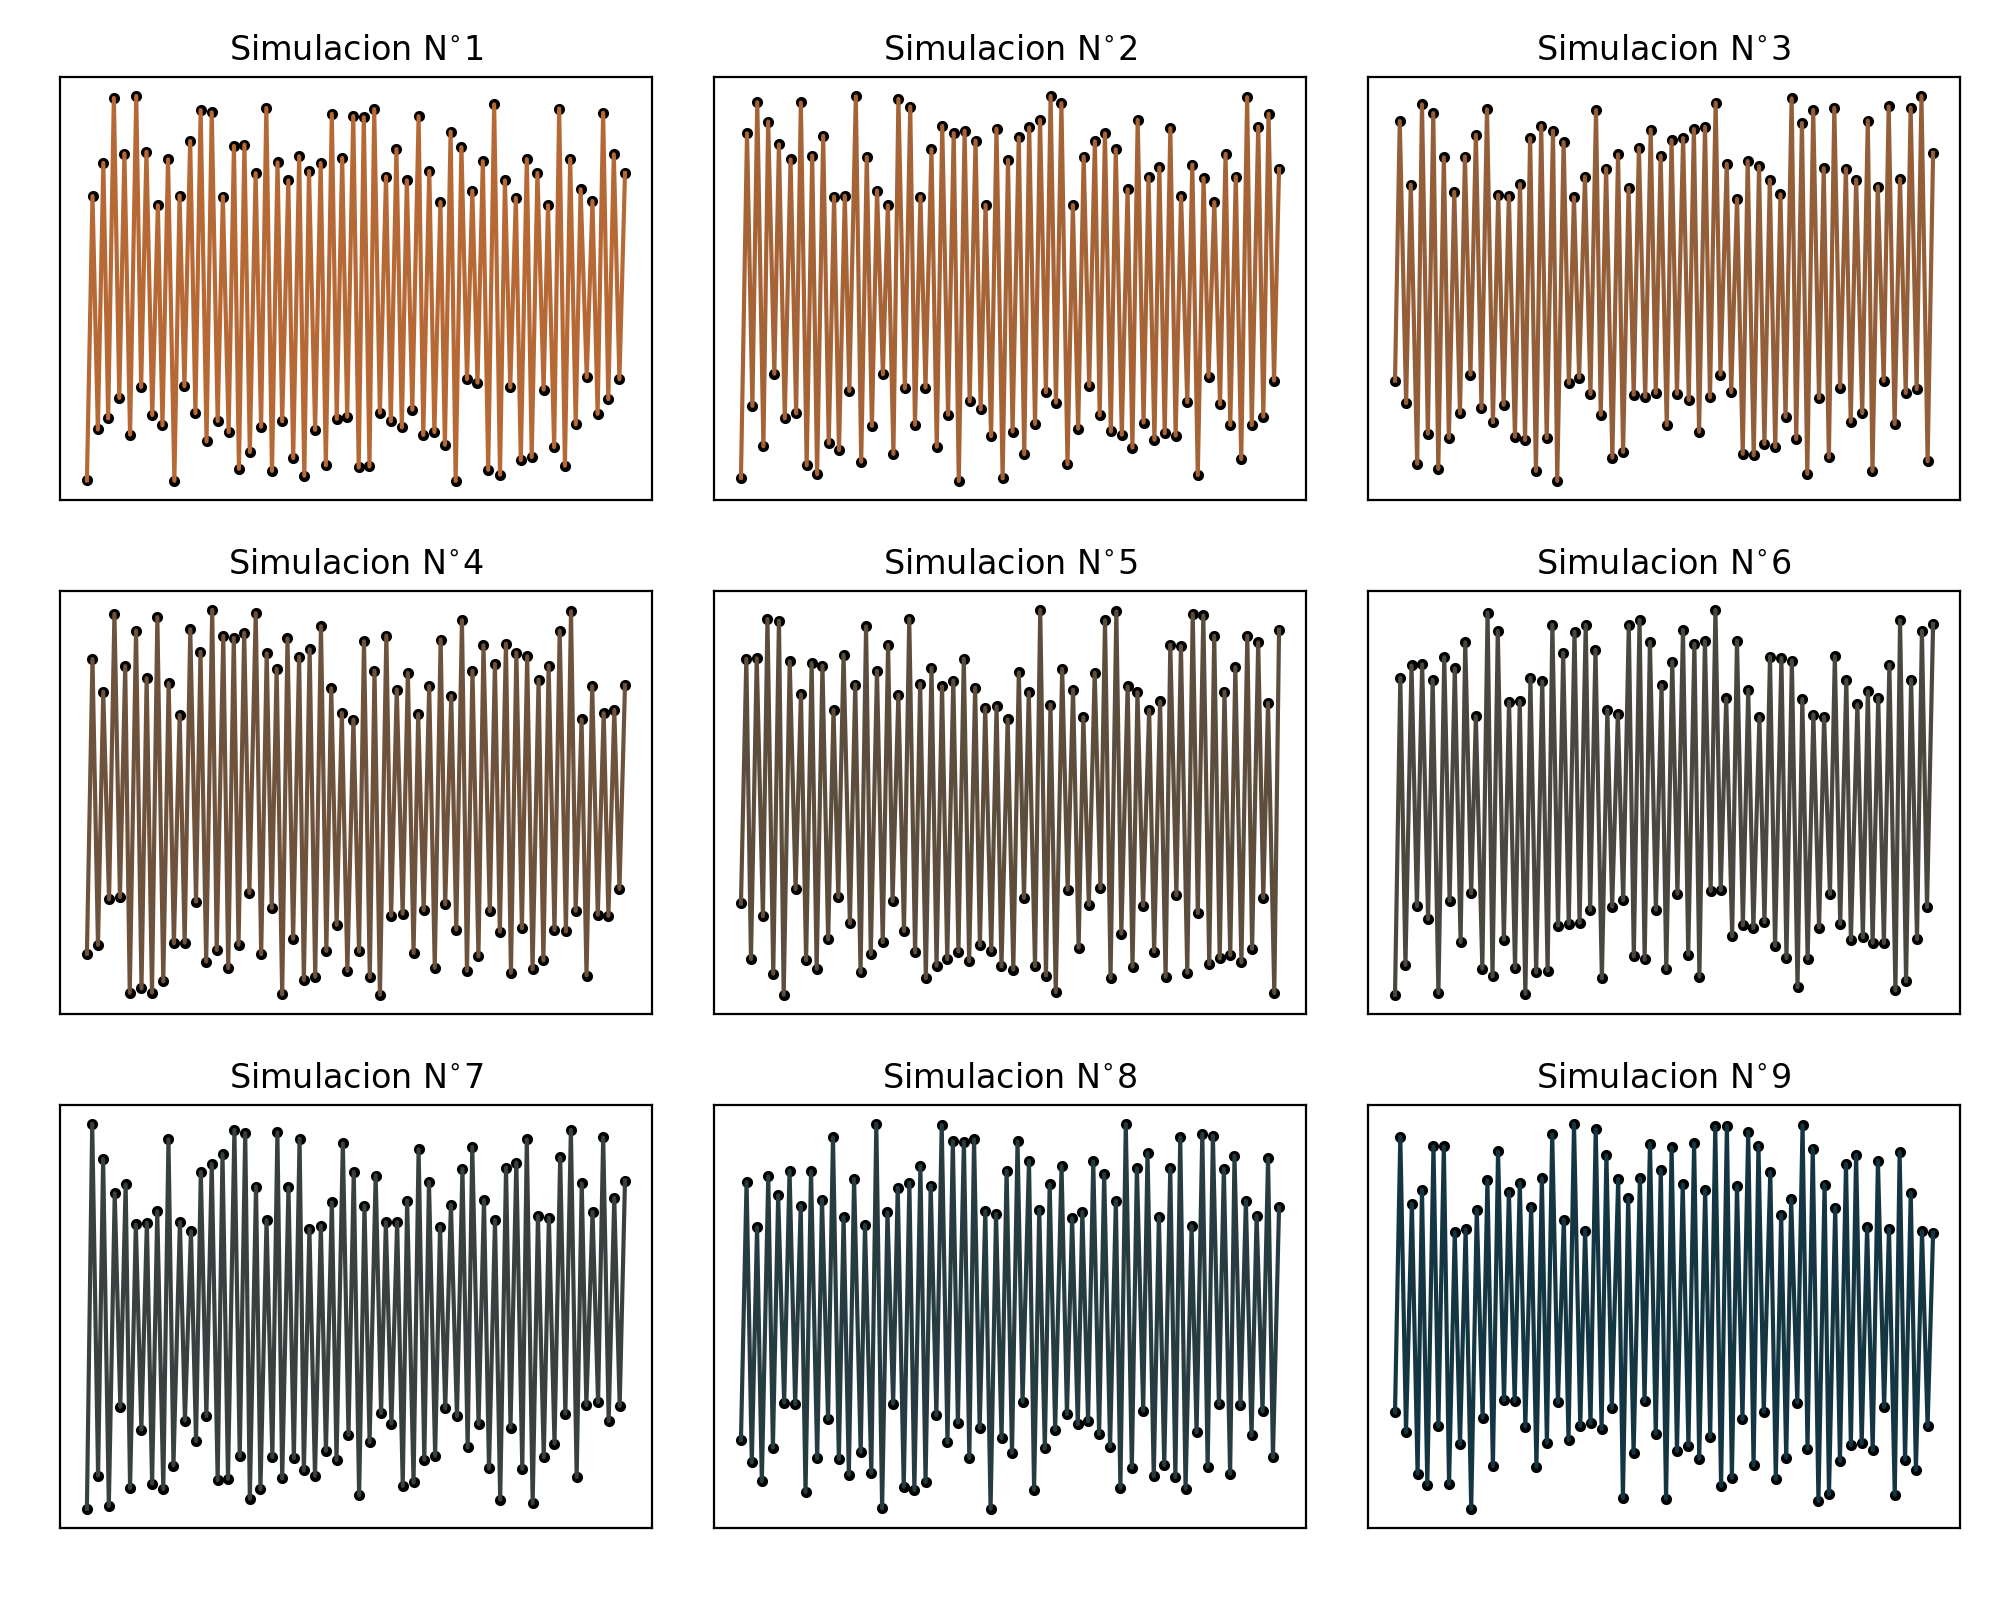
\includegraphics[scale=0.27]{../Graphics/pos_ini.png}
    \caption{Configuración inicial de las cadenas de moleculas.}
    \label{fig:posini}
\end{figure}
Las velocidades de cada molecula fueron dada siguiendo las siguientes ecuaciones:
\begin{align*}
    v_{xi}&=v_{0}\cos(2v_0\pi)\\
    v_{yi}&=v_{0}\sin(2v_0\pi)\\
\end{align*}
donde $v_0$ es un número aleatorio entre 0 y 1. Los parámetros usados para cada simulación son los que se muestran en la tabla \ref{table:parametros},
la dinámica que presento cada simulación estan guardadas en el siguiente link (\href{https://github.com/giovannilopez9808/Notas_Agosto_2020/tree/master/Simulaciones/Proyecto_4/Graphics/simulaciones}{simulaciones.mp4}).
En cada una de ellas se realizó la monitorización de la energía potencial, energía cinética y las posiciones de cada molecula. En la figura \ref{fig:dim}
se visualiza como es la evolución a diferentes tiempos de una simulación.
\begin{figure}[H]
    \centering
    \hspace{-0.5cm}
    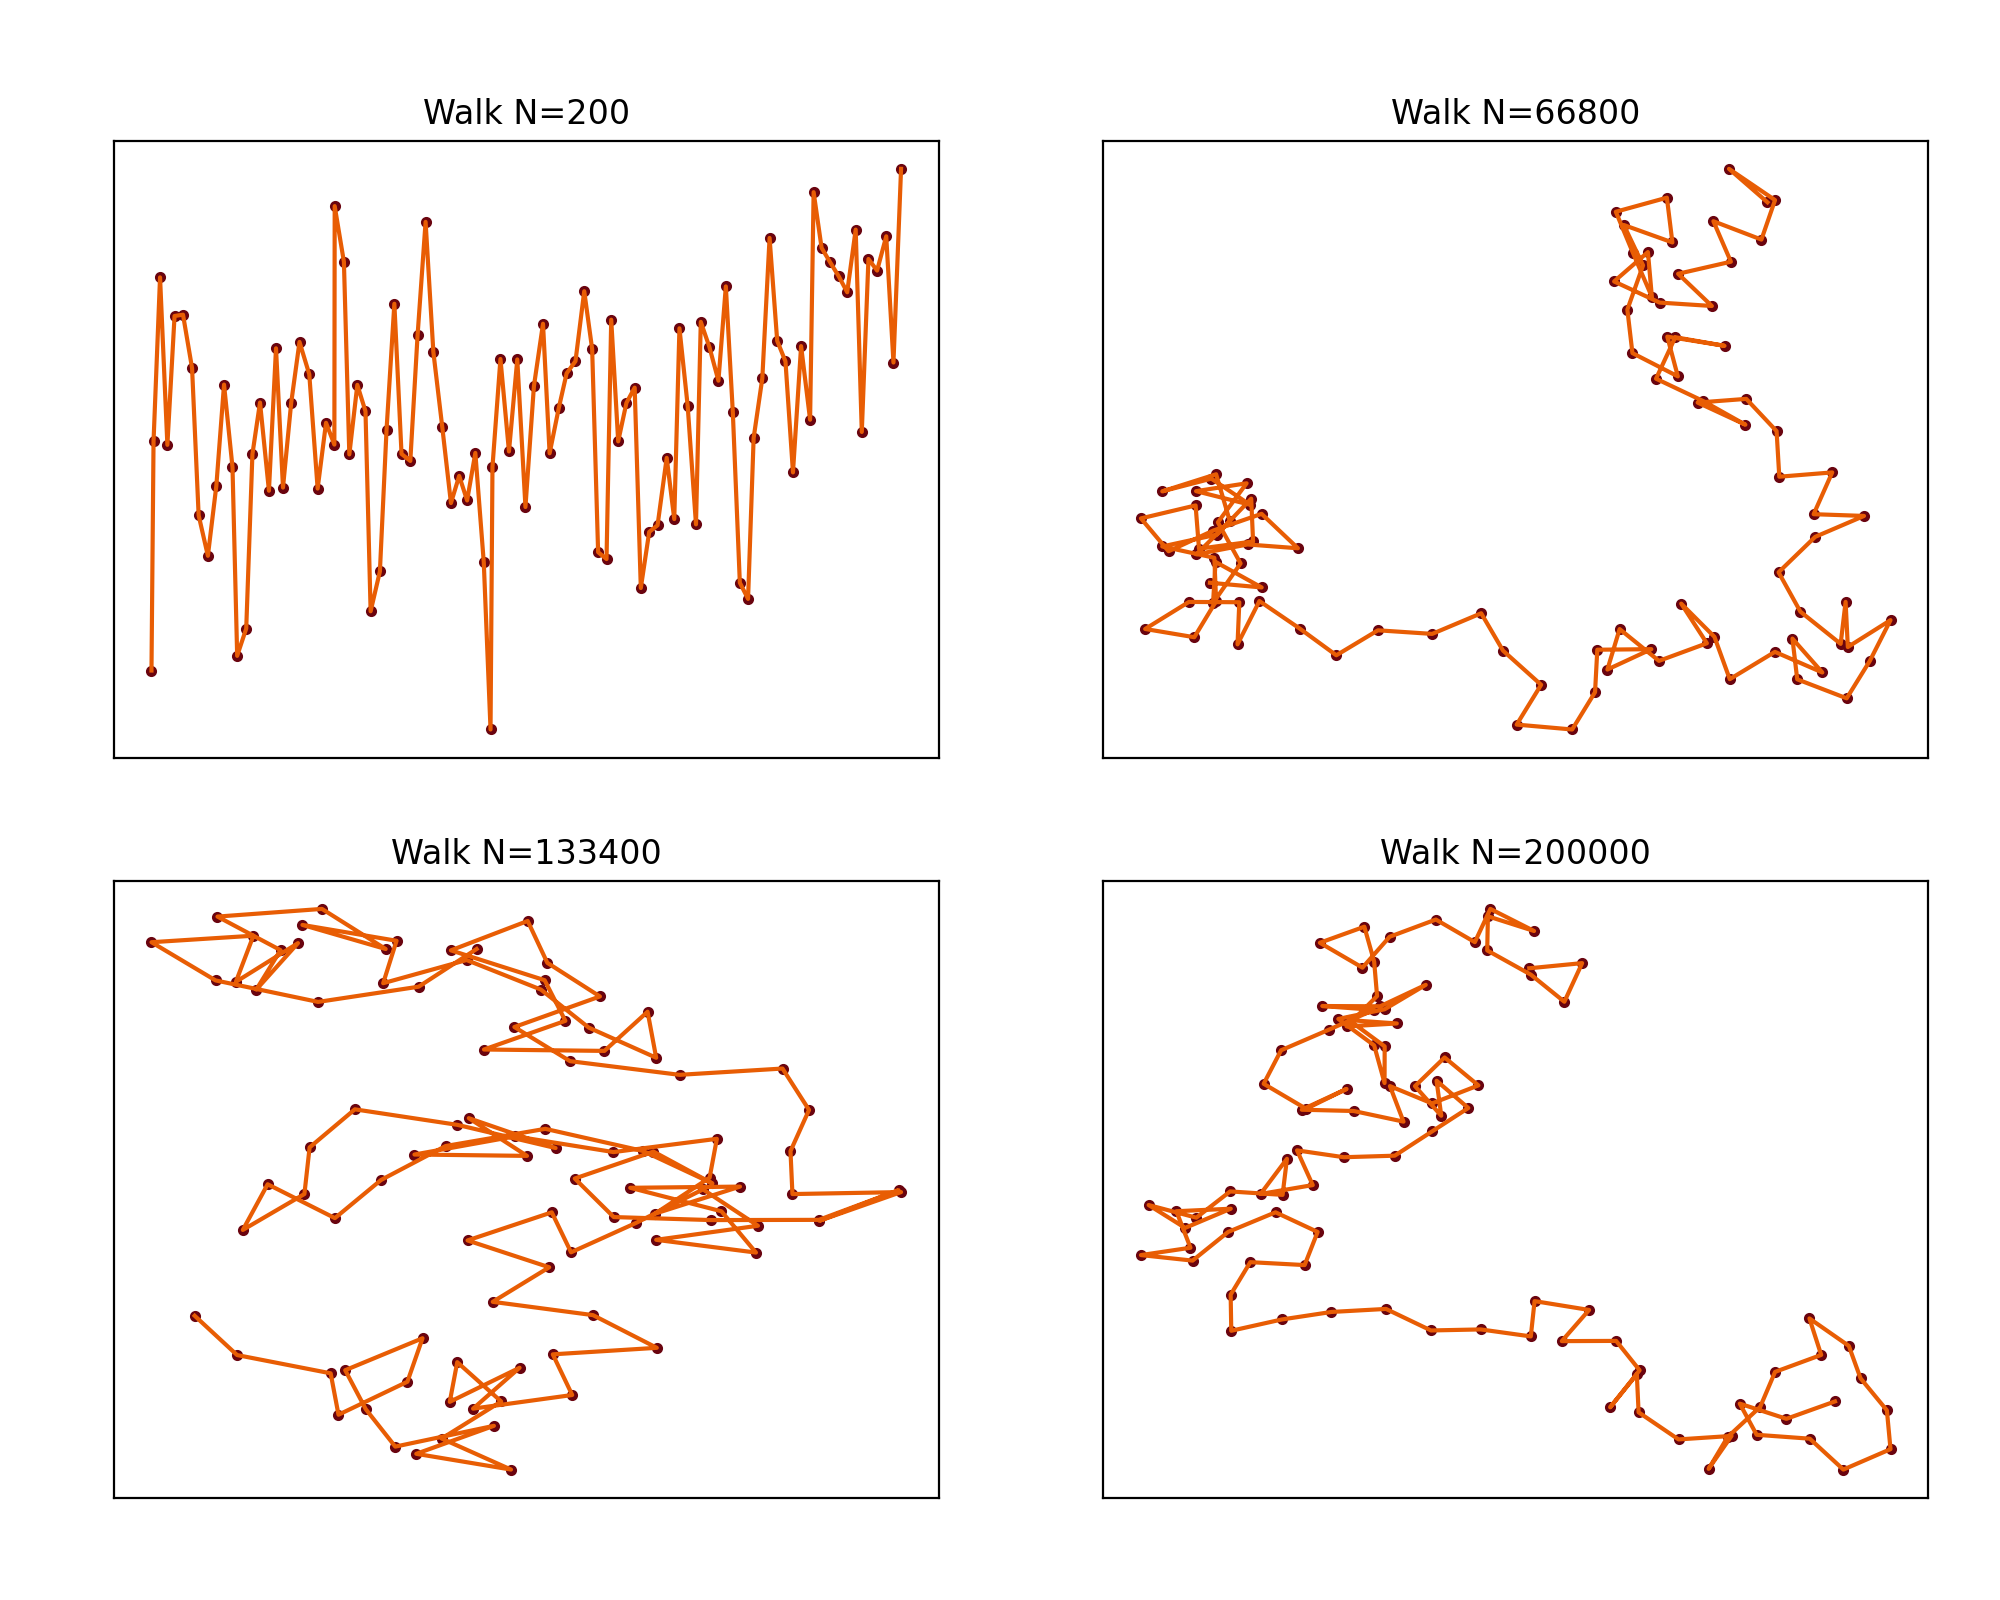
\includegraphics[scale=0.3]{../Graphics/dim.png}
    \caption{Dinámica de una simulación de la cadena de moleculas a diferentes tiempos.}
    \label{fig:dim}
\end{figure}
Realizando el calculo de la temperatura del sistema a cada paso de la simulación se obtuvo la figura \ref{fig:temp}.
\begin{figure}[H]
    \centering
    \hspace{-0.2cm}
    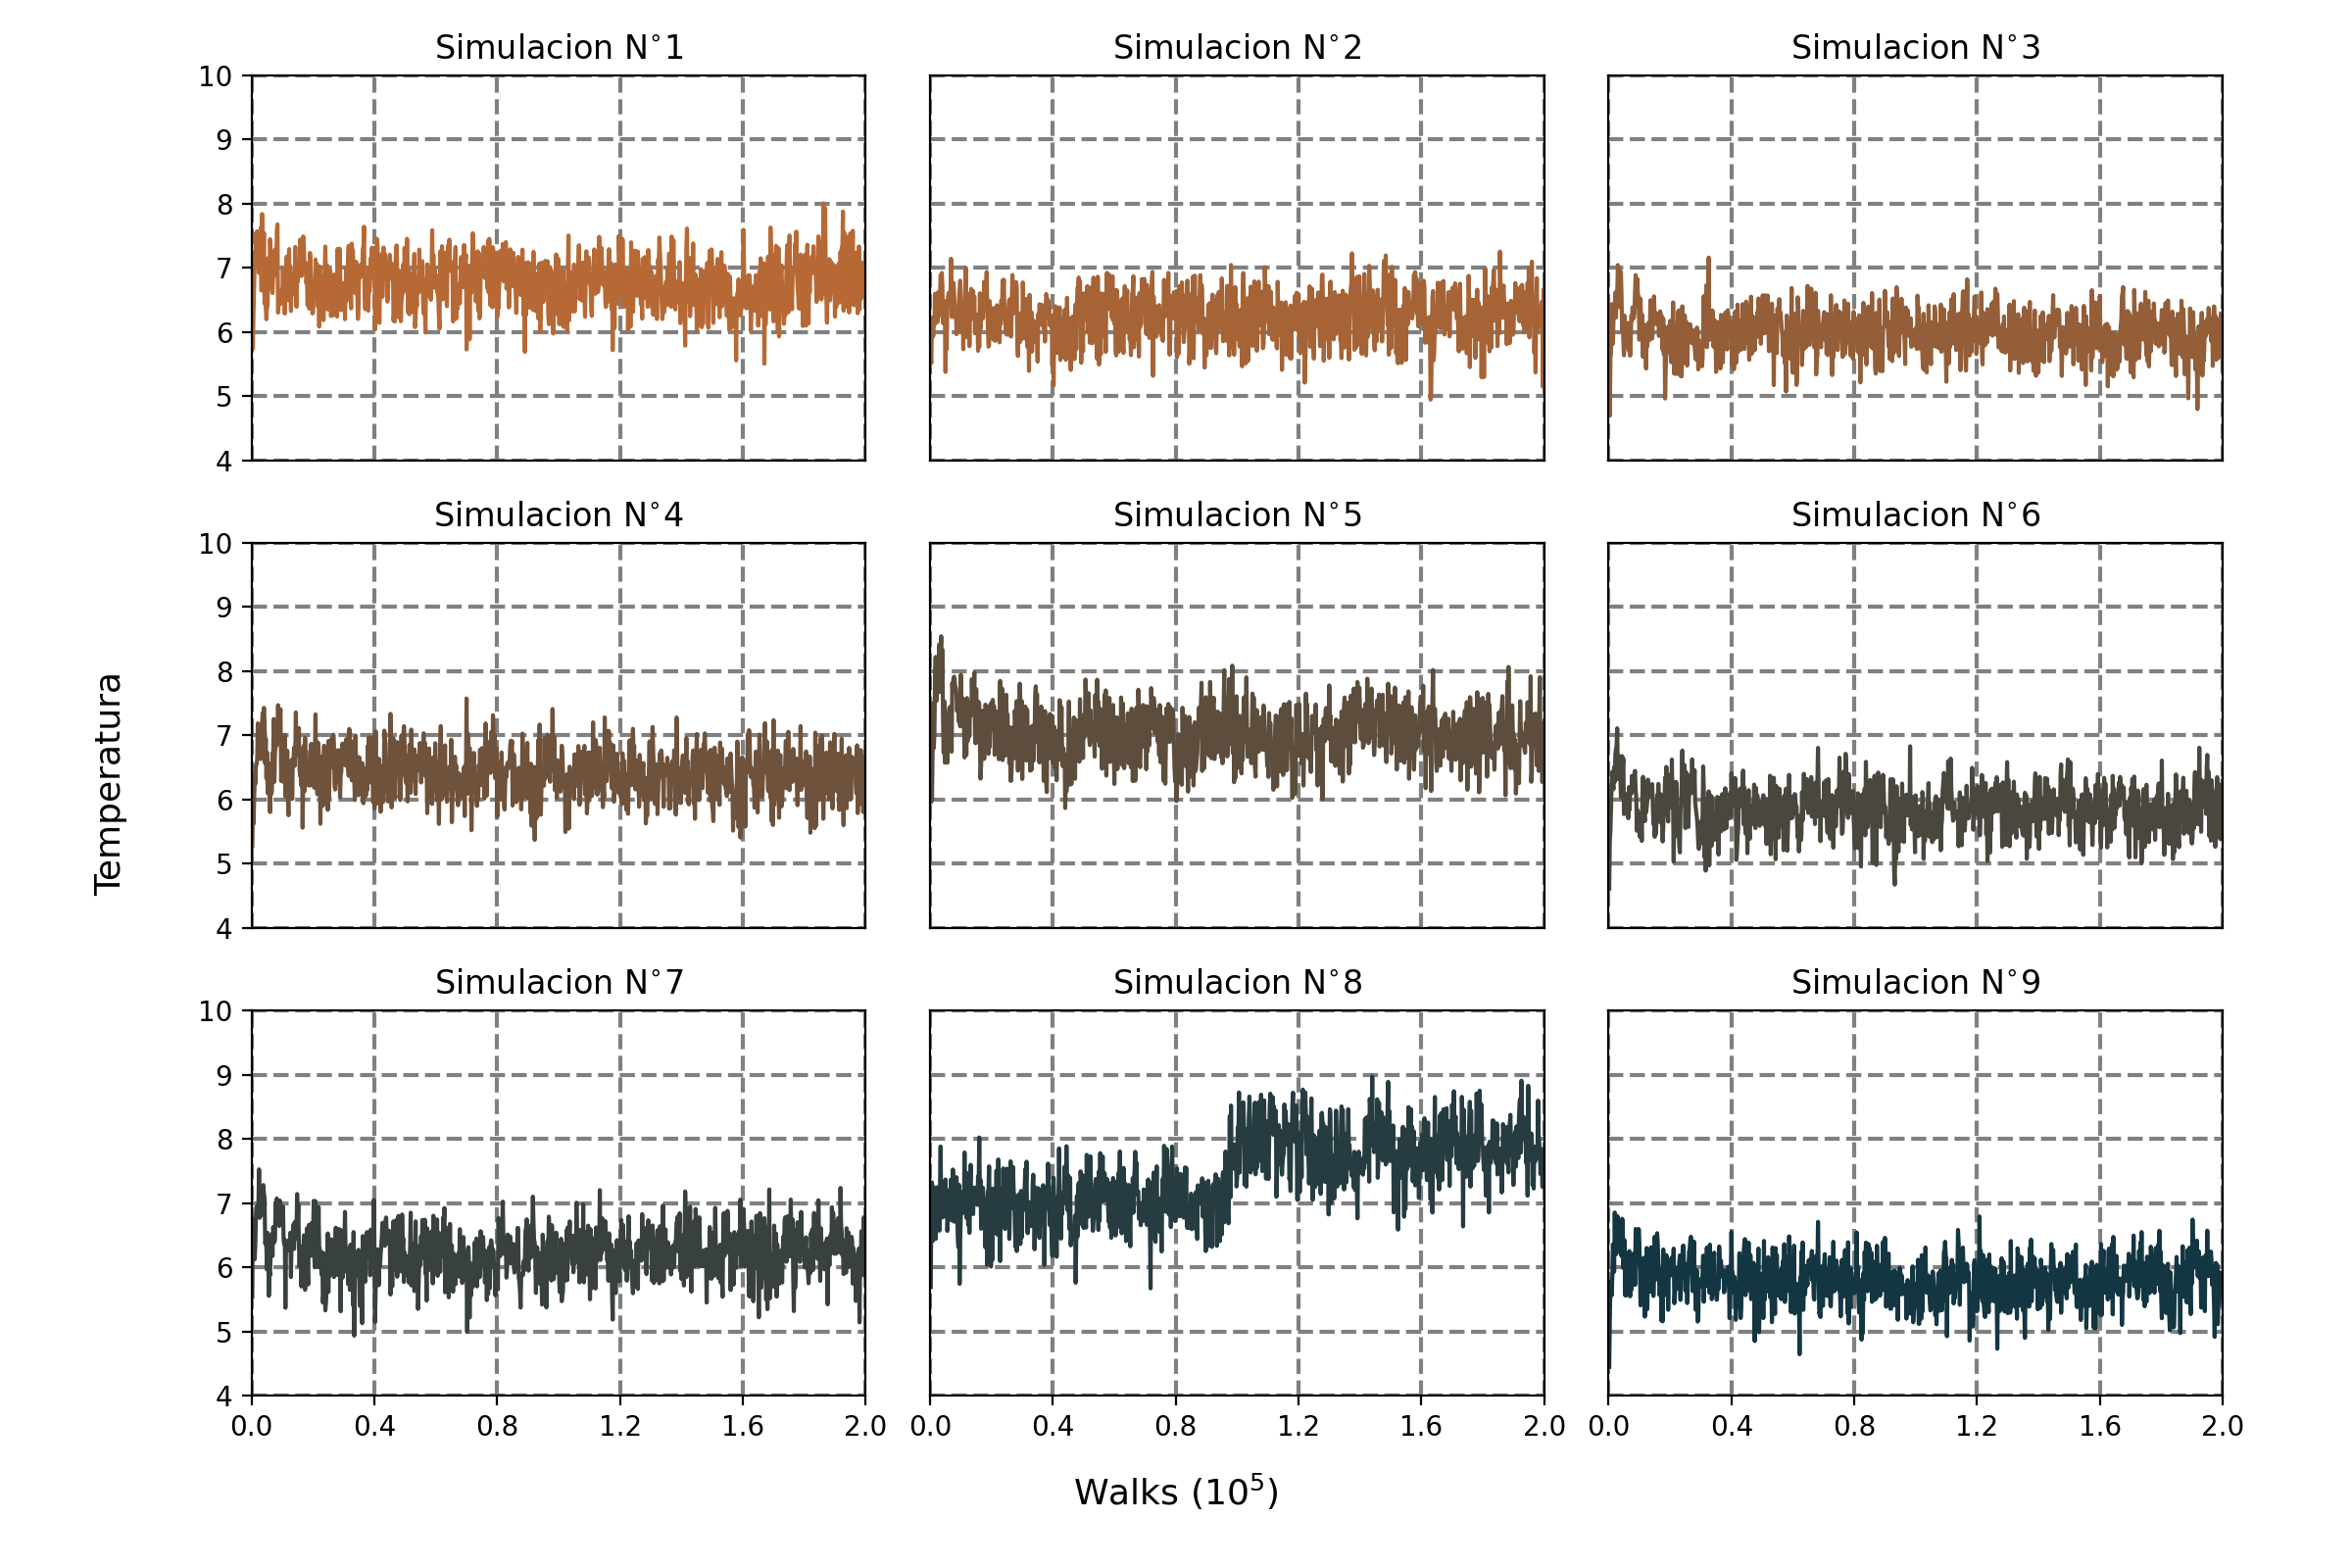
\includegraphics[scale=0.25]{../Graphics/temp.png}
    \caption{Temperatura de las diferentes simulaciones de la cadena de moleculas bajo el potencial de Lennard-Jones y el potencual FENE.}
    \label{fig:temp}
\end{figure}
Y observando la variación de la energía potencial a lo largo de la simulación se obtuvo la figura \ref{fig:energy}.
\begin{figure}[H]
    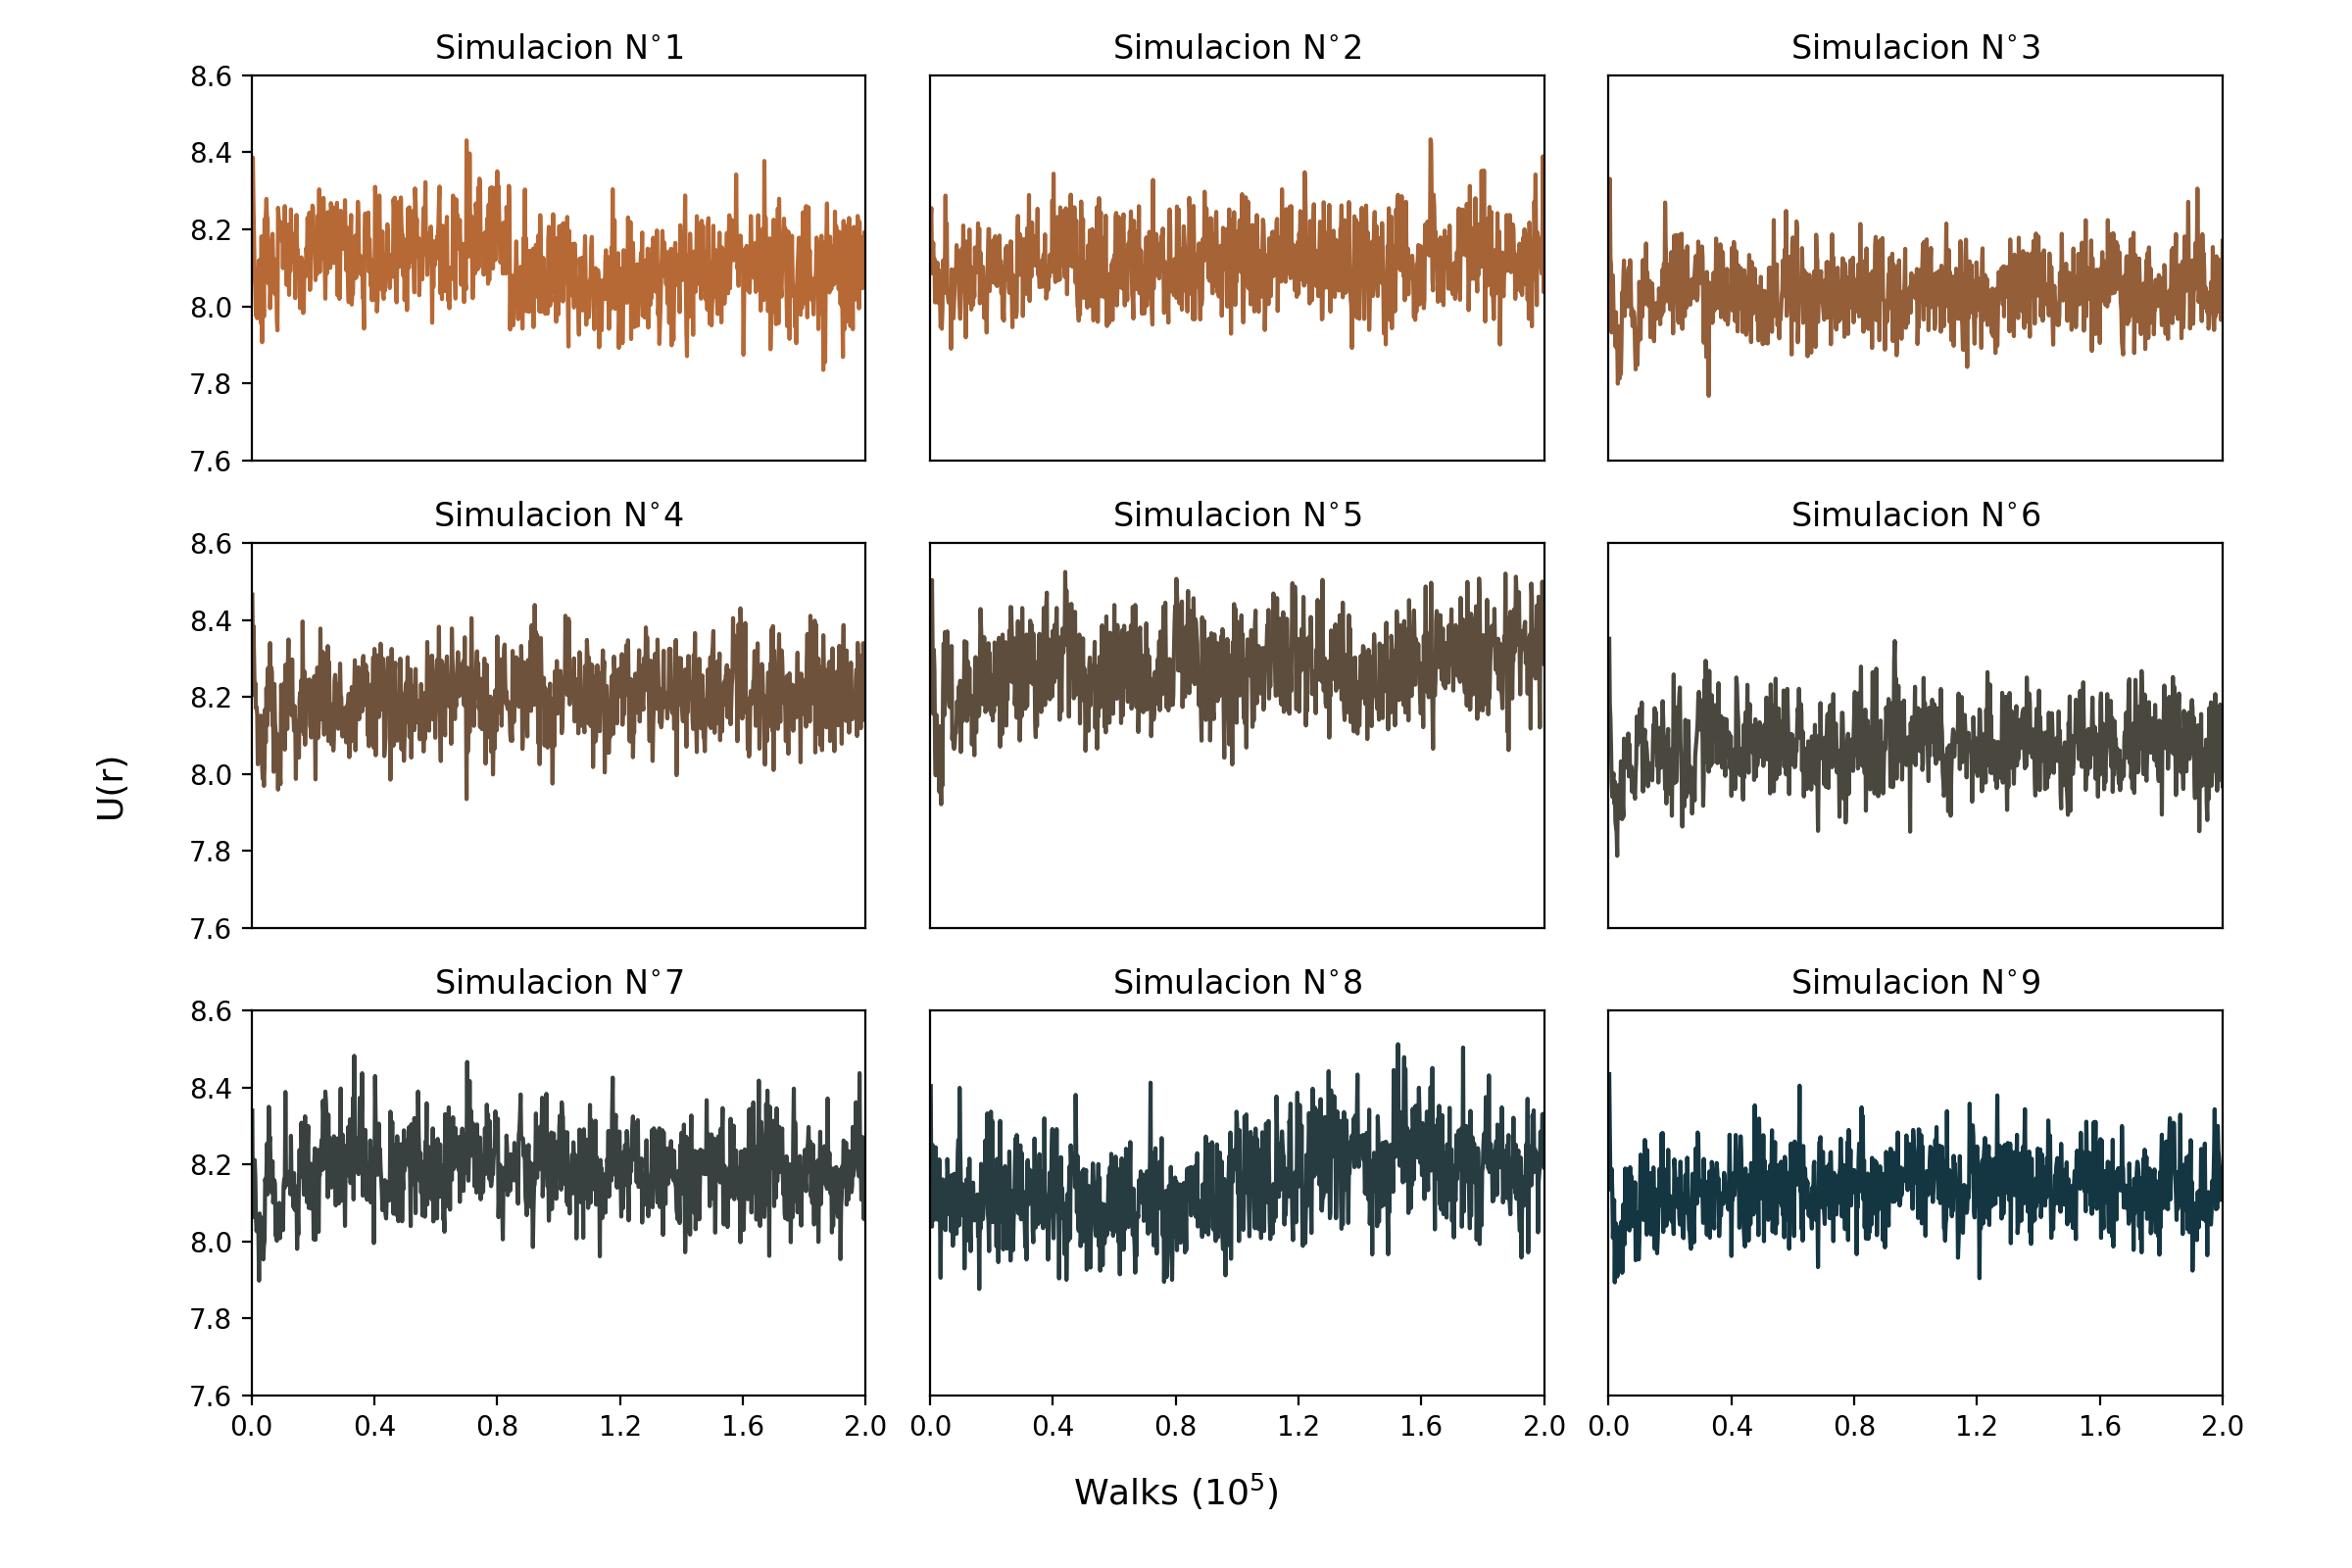
\includegraphics[scale=0.25]{../Graphics/energy.png}
    \caption{Energía potencial de las diferentes simulaciones de la cadena de moleculas bajo el potencial de Lennard-Jones y el potencual FENE}
    \label{fig:energy}
\end{figure}
Obteniendo un valor medio de la temperatura y la energía potencial se obtiene la tabla \ref{table:mean}.
\begin{table}[H]
    \centering
    \begin{tabular}{ccc} \hline
        Simulación & $\bar{U}(r)$ & $\bar{T}$ \\ \hline
        1&0.0811&0.0068\\
        2&0.0811&0.0063\\
        3&0.0804&0.006\\
        4&0.082&0.0064\\
        5&0.0827&0.007\\
        6&0.0807&0.0059\\
        7&0.0819&0.0062\\
        8&0.0815&0.0074\\
        9&0.0814&0.0058\\ \hline
    \end{tabular}
    \caption{Valores medios de la energía potencial $(\bar{U}(r))$ y la temperatura $(\bar{T})$ en cada simulación realizada.}
    \label{table:mean}
\end{table}